\documentclass[../Cours.tex]{subfiles}
\usepackage{multicol}

\begin{document}

\begin{luacode}
    function nom_prefixe(exposant_prefixe)
        if exposant_prefixe == 15 then return "peta" end
        if exposant_prefixe == 12 then return "tera" end
        if exposant_prefixe == 9 then return "giga" end
        if exposant_prefixe == 6 then return "mega" end
        if exposant_prefixe == 3 then return "kilo" end
        if exposant_prefixe == 2 then return "hecto" end
        if exposant_prefixe == 1 then return "deca" end
        if exposant_prefixe == -1 then return "deci" end
        if exposant_prefixe == -2 then return "centi" end
        if exposant_prefixe == -3 then return "milli" end
        if exposant_prefixe == -6 then return "micro" end
        if exposant_prefixe == -9 then return "nano" end
        if exposant_prefixe == -12 then return "pico" end
        if exposant_prefixe == -15 then return "femto" end
    end

    function prefixe(exposant_prefixe)
        if exposant_prefixe == 0 then return "" end
        return "\\" .. nom_prefixe(exposant_prefixe)
    end

    function parenthese_nombre_negatif(n)
        if n < 0 then return "(-" .. math.abs(n) .. ")" 
        else return math.abs(n) end
    end

    function combinaison_puissance(a, b)
        local aa = parenthese_nombre_negatif(a)
        local bb = parenthese_nombre_negatif(b)
        local cc = parenthese_nombre_negatif(a+b)
        return "(on combine les puissances de 10 $\\Rightarrow " .. aa .. " + " .. bb .. " = " .. cc .. "$)"
    end  
    
    function conversion_puissances(nombre, unite, exposant_prefixe1, exposant_prefixe2)
        tex.print("Convertir \\qty{".. nombre .. "}{" .. prefixe(exposant_prefixe1) .. unite .. "} en \\unit{" .. prefixe(exposant_prefixe2) .. unite .. "}\\\\")
        tex.print("\\renewcommand{\\arraystretch}{1.65}")
        tex.print("\\begin{tabularx}{\\linewidth}{{>{$}l<{$}}R}")

        local i = string.find(nombre, "e")
        local num = tonumber(string.sub(nombre, 1, i-1))
        local expo = tonumber(string.sub(nombre, i+1, -1))

        -- étape 0 : énoncé
        local afficher_expo = "\\times 10^{" .. expo .. "}"
        if expo == 0 then afficher_expo = "" end
        tex.print("\\textcolor{rouge}{\\num{" .. num .. "}} " .. afficher_expo .. "~\\unit{" .. prefixe(exposant_prefixe1) .. unite .. "}&\\\\")

        local decal = math.floor(math.log(num, 10))
        local direction = "droite"
        if decal < 0 then direction = "gauche" end 
        local mantisse = num / math.pow(10,decal)

        if decal ~= 0 then
            if expo ~= 0 then
                -- étape 1 : passage à l'écriture scientifique
                tex.print("=\\textcolor{rouge}{\\num{" .. mantisse .. "} \\times 10^{" .. decal .. "}} \\times 10^{" .. expo .. "}~\\unit{" .. prefixe(exposant_prefixe1) .. unite  .."} & \\makecell[l]{\\textcolor{rouge}{(passage à l'écriture scientifique :} \\\\ \\textcolor{rouge}{la virgule est décalée " .. math.abs(decal) .. " fois vers la " .. direction .. " $\\Rightarrow \\times 10^{" .. decal .. "}$)}}\\\\")
        
                -- étape 2 : combinaison des puissances
                tex.print("=\\num{" .. mantisse .. "} \\times 10^{" .. expo + decal .. "}~\\unit{\\textcolor{vert}{" .. prefixe(exposant_prefixe1) .. "}" .. unite .. "}&" .. combinaison_puissance(decal, expo) .. "\\\\")
                expo = expo + decal
            else
                -- étape 1 : passage à l'écriture scientifique
                tex.print("=\\textcolor{rouge}{\\num{" .. mantisse .. "} \\times 10^{" .. decal .. "}}~\\unit{\\textcolor{vert}{" .. prefixe(exposant_prefixe1) .. "}" .. unite  .."} & \\makecell[l]{\\textcolor{rouge}{(passage à l'écriture scientifique :} \\\\ \\textcolor{rouge}{la virgule est décalée " .. math.abs(decal) .. " fois vers la " .. direction .. " $\\Rightarrow \\times 10^{" .. decal .. "}$)}}\\\\")
                expo = decal
            end
        end

        afficher_expo = "\\times 10^{" .. expo .. "}"
        if expo == 0 then afficher_expo = "" end

        if exposant_prefixe1 ~= 0 then
            -- étape 3 : remplacement du préfixe
            tex.print("=\\num{" .. mantisse .. "}" .. afficher_expo .. " \\times \\textcolor{vert}{10^{" .. exposant_prefixe1 .. "}}~\\unit{" .. unite .. "}&(dans la tableau, \\textcolor{vert}{" .. nom_prefixe(exposant_prefixe1) .. " vaut $10^{" .. exposant_prefixe1 .. "}$})\\\\")
    
            if expo ~= 0 then
                -- étape 4 : combinaison des puissances
                tex.print("=\\num{" .. mantisse .. "} \\times 10^{" .. expo + exposant_prefixe1 .. "}~\\unit{" .. unite .. "}&" .. combinaison_puissance(expo, exposant_prefixe1) .. "\\\\")
                expo = expo + exposant_prefixe1
            end
            expo = exposant_prefixe1
        end

        afficher_expo = "\\times 10^{" .. expo .. "}"
        if expo == 0 then afficher_expo = "" end

        if exposant_prefixe2 ~= 0 then 
            -- étape 5 : ajout du nouveau préfixe
            tex.print("=\\num{" .. mantisse .. "}" .. afficher_expo .. " \\times \\textcolor{bleu}{10^{" .. -exposant_prefixe2 .. "}}~\\unit{\\textcolor{bleu}{" .. prefixe(exposant_prefixe2) .. "}" .. unite .. "}&(dans la tableau, \\qty{1}{" .. prefixe(exposant_prefixe2) .. unite .. "} vaut $10^{" .. exposant_prefixe2 .. "}$~\\unit{" .. unite .. "}, \\textcolor{bleu}{donc \\qty{1}{" .. unite .."} vaut $10^{" .. -exposant_prefixe2 .. "}$~\\unit{" .. prefixe(exposant_prefixe2) .. unite .. "}})\\\\")

            if expo ~= 0 then
                -- étape 6 : combinaison des puissances
                tex.print("=\\num{" .. mantisse .. "} \\times 10^{" .. expo - exposant_prefixe2 .. "}~\\unit{" .. prefixe(exposant_prefixe2) .. unite .. "}&" .. combinaison_puissance(expo, -exposant_prefixe2) .. "\\\\")
                expo = expo - exposant_prefixe2
            end
        end
        
        tex.print("\\end{tabularx}")
        tex.print("\\renewcommand{\\arraystretch}{1}")
    end
\end{luacode}

%%%%%%%%%%%%%%%%%%%%%%%%%%%%%%%%%%%%%%%%%%%%%%%%%%%%%%%%%%%%%%%%%%%%%

\chapitre{Puissances}

\partie{Les puissances de 10}
\souspartie{De la multiplication aux puissances}

\definition{Soit $n$ un nombre entier positif non nul. \\$10^n$ (se lit << 10 puissance $n$ >>) est le produit de $n$ facteurs égaux à 10.}

\exemple{%
\begin{itemize}%
    \item $10^9 = \textcolor{vert}{10 \times 10 \times 10 \times 10 \times 10 \times 10 \times 10 \times 10 \times 10} = \num{1000000000}$
    \item $10^4 = \textcolor{vert}{10 \times 10 \times 10 \times 10} = \num{10000}$
    \item $10^5 = \textcolor{vert}{10 \times 10 \times 10 \times 10 \times 10} = \num{100000}$
    \item $10^2 = \textcolor{vert}{10 \times 10} = \num{100}$
    \item $10^0 = 1$
\end{itemize}%
}

\formule{$$10^{-n} = \dfrac{1}{10^n} ~~~~~~ 10^n \times 10^p = 10^{n+p} ~~~~~~ \dfrac{10^n}{10^p} = 10^{n-p} ~~~~~~ \left(10^n\right)^p = 10^{n\times p} $$}

\begin{listedexemples}
\begin{multicols}{2}
    \item $10^{-2} = \dfrac{1}{10^2} = \dfrac{1}{100} = 0,01$
    \item $10^3\times 10^2 = 10^{3+2} = 10^5$
    \item $10^2 \times 10^4 = 10^{2+4} = 10^6$
    \item $\dfrac{10^4}{10^1} = 10^{4-1} = 10^3$
    \item $10^{-5} = \dfrac{1}{10^5} = \dfrac{1}{\num{100000}} = \num{0,00001}$
    \item $10^3 \times 10^{-2} = 10^{3 + (-2)} = 10^1$
    \item $\left(10^2\right)^3 = 10^{2 \times 3} = 10^6$
    \item $\left(10^4\right)^{-2} = 10^{4 \times (-2)} = 10^{-8}$ 
\end{multicols}
\end{listedexemples}


\clearpage
\souspartie{Écriture scientifique d'un nombre décimal}

\methode{Soit $n$ un nombre entier positif.
\begin{itemize}
    \item Multiplier un nombre par $10^n$, c'est décaler la virgule de $n$ chiffres vers la droite.
    \item Multiplier un nombre par $10^{-n}$, c'est décaler la virgule de $n$ chiffres vers la gauche.
\end{itemize}}

\begin{listedexemples}
\begin{multicols}{2}
\begin{luacode}
    function decalage_virgule(nombre, decal)
        local res = nombre * math.pow(10, decal)
        if res == math.floor(res) then res = math.floor(res) end
        tex.print("$\\num{" .. nombre .. "} \\times 10^{" .. decal .. "} = \\num{" .. res .. "}$")
    end
    item() decalage_virgule(1.234, 2)
    item() decalage_virgule(96.76, -3)
    item() decalage_virgule(39.42649, 4)
    item() decalage_virgule(0.003825, -1)
    item() decalage_virgule(1.9274, 5)
    item() decalage_virgule(10.218, -3)
\end{luacode}
\end{multicols}
\end{listedexemples}

\remarque{Un nombre décimal peut s'écrire de plusieurs façons à l'aide de puissances de 10.}

\definition{L'écriture scientifique d'un nombre décimal non nul ($\neq 0$) est \emph{l'unique} écriture de la forme $a \times 10^n$ où :
\begin{itemize}
    \item $a$ est un nombre décimal n'ayant qu'un chiffre autre que 0 avant la virgule, c'est-à-dire $1 \infeg a < 10$
    \item $n$ est un nombre entier relatif
\end{itemize}}

\begin{listedexemples}
\begin{multicols}{2}
\begin{luacode}
    function ecriture_scientifique(nombre)
        local exposant = math.floor(math.log(nombre, 10))
        local res = nombre / math.pow(10, exposant)
        tex.print("$\\num{" .. nombre .. "} = \\num{" .. res .. "} \\times 10^{" .. exposant .. "}$")
    end
    item() ecriture_scientifique(120546)
    item() ecriture_scientifique(0.436)
    item() ecriture_scientifique(540000)
    item() ecriture_scientifique(0.00876)
    item() ecriture_scientifique(0.0715)
    item() ecriture_scientifique(12.34)
    item() ecriture_scientifique(0.00016)
    item() ecriture_scientifique(6.725)
\end{luacode}
\end{multicols}
\end{listedexemples}

\clearpage
\souspartie{Système International (SI)}

\underline{Tableau des préfixes du SI :}

\color{noir}
{
\setlength{\tabcolsep}{0pt}
\tiny
\newcommand*\rot{\rotatebox{90}}
\begin{center}
\begin{tabularx}{\textwidth}{|*{21}{C|}}\hline
    \multicolumn{3}{|c}{Milliards} & \multicolumn{3}{|c}{Million} & \multicolumn{3}{|c}{Milliers} & \multicolumn{3}{|c}{Unité} & \multicolumn{3}{|c}{Millièmes} & \multicolumn{3}{|c}{Millionièmes} & \multicolumn{3}{|c|}{Milliardièmes}  \\\hline
    & & giga & & & méga & & & kilo & hecto & déca & & déci & centi & milli & & & micro & & & nano \\\hline
    & & $G$ & & & $M$ & & & $k$ & $h$ & $da$ & & $d$ & $c$ & $m$ & & & $\mu$ & & & $n$\\\hline
    & & $10^9$ & \hspace{-3em}\phantom{$10^{1^2}$}& & $10^6$ & & & $10^3$ & $10^2$ & $10^1$ & $10^0$ & $10^{-1}$ & $10^{-2}$ & $10^{-3}$ & & & $10^{-6}$ & & & $10^{-9}$ \\\hline
    \rot{centaines de milliards} & \rot{dizaines de milliards} & \rot{milliards} & \rot{centaines de millions} & \rot{dizaines de millions} & \rot{millions} & \rot{centaines de milliers} & \rot{dizaines de milliers} & \rot{milliers} & \rot{centaines} & \rot{dizaines} & \rot{unités} & \rot{dixièmes} & \rot{centièmes} & \rot{millièmes} & \rot{dix-millièmes} & \rot{cent-millièmes} & \rot{millionièmes} & \rot{dix-millionièmes} & \rot{cent-millionièmes} & \rot{milliardièmes} \\\hline
\end{tabularx}
\end{center}
}

\underline{Tableau des sept unités de base du SI :}

\begin{center}
\begin{tabularx}{\textwidth}{|X|c|c|}\hline
    Grandeur physique & Unité & Symbole de l'unité\\\hline
    masse & kilogramme & kg\\
    longueur & mètre & m\\
    temps & seconde & s\\
    température thermodynamique & kelvin & K\\
    intensité du courant électrique & ampère & A\\
    quantité de matière & mole & mol\\
    intensité lumineuse & candela & cd\\\hline
\end{tabularx}
\end{center}

\color{bleu}

\begin{listedexemples}
    \small
    \item[] \fbox{Cas n°1}
    \begin{luacode}
        item() conversion_puissances("1e0", "\\octet", 9, 0)
        item() conversion_puissances("30e0", "\\metre", 3, 0)
    \end{luacode}
    \clearpage
    \item[] \fbox{Cas n°2}
    \begin{luacode}
        item() conversion_puissances("5e0", "\\volt", 0, -3)
        item() conversion_puissances("101300e0", "\\pascal", 0, 2)
    \end{luacode}
    \item[] \fbox{Cas n°3}
    \begin{luacode}
        item() conversion_puissances("398.76e-6", "\\volt", -9, 9)
        item() conversion_puissances("0.00078e-1", "\\metre", -1, 1)
    \end{luacode}
\end{listedexemples}

\clearpage
\partie{Puissances à base quelconque}

\definition{Soit $a$ un nombre réel, \\
soit $n$ un entier naturel, 
$$a^n = \underbrace{a \times a \times ... \times a}_{\mbox{$n$ facteurs}}$$
$a$ est appelé la base\\
$n$ est appelé l'exposant}

\convention{Pour n'importe quelle base $a$ : $$a^0 = 1$$}

\formule{$$a^{-n} = \dfrac{1}{a^n} ~~~~~~ a^n \times a^p = a^{n+p} ~~~~~~ \dfrac{a^n}{a^p} = a^{n-p} ~~~~~~ \left(a^n\right)^p = a^{n\times p} $$}

\begin{listedexemples}
    \item $2^{-4} = \dfrac{1}{2^4}$
    \item $3^2 \times 3^7 = 3^9$
    \item $\dfrac{4^2}{4^8} = 4^{2-8} = 4^{-6}$
    \item $\left(5^2\right)^4 = 5^{2 \times 4} $
    \item $\dfrac{6^2 \times 6^3}{6^6} = \dfrac{6^{2+3}}{6^6} = \dfrac{6^5}{6^6} = 6^{5-6} = 6^{-1}$
    \item $\left( 7^2 \times 7^4 \right)^7 = \left(7^{2+4}\right)^7 = \left(7^6\right)^7 = 7^{6 \times 7} = 7^{42}$
\end{listedexemples}

\propriete{Pour tout nombre réel $x$, $x^2$ est positif}

\propriete{\begin{itemize}
    \item Un nombre négatif élevé à une puissance paire est positif.
    \item Un nombre négatif élevé à une puissance impaire est négatif.
\end{itemize}}

\begin{listedexemples}
    \item[*] $(-2)^5 < 0$
    \item[*] $(-6)^6 > 0$
    \item[*] $0^3 = 0$ (positif et négatif)
    \item[*] $7^3 > 0$ (la base est positive)
\end{listedexemples}


%%%%%%%%%%%% EXERCICES %%%%%%%%%%%%%%%%
\clearpage
\EXERCICES
\begin{questions}
    \exercicetitre{Écrire les nombres suivants avec la notation scientifique}\vspace{-1.5em}
        \begin{multicols}{2}
            \question $\num{34,5} = $
            \question $\num{17,897654} =$
            \question $\num{0,0000123} =$
            \question $\num{9823,12} =$
            \question $\num{0,100234010} =$
            \question $\num{2871,9273} =$
        \end{multicols}

    \exercicetitre{Écrire les nombres suivants avec l'écriture décimale}\vspace{-1.5em}
        \begin{multicols}{2}
            \question $4,2 \times 10^3 = $
            \question $6,07 \times 10^{-2} =$
            \question $4,23 \times 10^2 =$
            \question $8,923 \times 10^{-3} =$
            \question $9,98 \times 10^{2} = $
            \question $2 \times 10^{6} = $
        \end{multicols}

    \exercicetitre{Convertir les quantités suivantes en mètres}\vspace{-1.5em}
        \begin{multicols}{2}
            \question $\qty{4,2}{\kilo\metre} =$
            \question $\qty{2,5}{\giga\metre} =$
            \question $\qty{9,8}{\milli\metre} =$
            \question $\qty{8,1}{\nano\metre} =$
        \end{multicols}

    \exercicetitre{Convertir les quantités suivantes selon l'unité demandée}\vspace{-1.5em}
        \begin{multicols}{2}
            \question $\qty{2,3}{\metre} \mbox{~en~} \unit{\centi\metre}$
            \question $\qty{0,02}{\metre} \mbox{~en~} \unit{\kilo\metre}$
            \question $\qty{0,002}{\metre} \mbox{~en~} \unit{\nano\metre}$
            \question $\qty{18,258}{\metre} \mbox{~en~} \unit{\mega\metre}$
            \question $\qty{0,035}{\metre} \mbox{~en~} \unit{\deca\metre}$
            \question $\qty{9275,729}{\metre} \mbox{~en~} \unit{\hecto\metre}$
        \end{multicols}

    \exercicetitre{Convertir les quantités suivantes}\vspace{-1.5em}
        \begin{multicols}{2}
            \question $\qty{398.76e-6}{\nano\volt}$ en \unit{\giga\volt}
            \question $\qty{0.00078e-1}{\deci\metre}$ en \unit{\deca\metre}
            \question $\qty{1.35e-9}{\mega\gram}$ en \unit{\centi\gram}
            \question $\qty{0.00056e-5}{\kilo\metre}$ en \unit{\nano\metre}
            \question $\qty{1.0058e-9}{\micro\watt}$ en \unit{\hecto\watt}
            \question $\qty{9.61e18}{\milli\metre}$ en \unit{\mega\metre}
            \question $\qty{49005.4e7}{\micro\litre}$ en \unit{\centi\litre}
            \question $\qty{8.56e9}{\nano\metre}$ en \unit{\giga\metre}
        \end{multicols}

    \exercicetitre{Calculs entre nombres en écriture scientifique}\vspace{-1.5em}
        \begin{multicols}{2}
            \question $\num{2e5} \times \num{7.5e6} = $
            \question $\dfrac{\num{3.5e-6}}{\num{14e-2}} = $
            \question $\num{13e21} + \num{2e19} = $
            \question $\num{4.8e-10} - \num{2e-11} = $
        \end{multicols}

    \exercice
        $ABCD$ est un carré tel que $AB = \qty{4e25}{\milli\metre}$.\\
        $EFGH$ est un rectangle tel que $EF = \qty{8,9e24}{\milli\metre}$ et $EG = \qty{2,5e25}{\milli\metre}$.
        \question Entre $ABCD$ et $EFGH$, lequel a la plus grande aire ?
        \question Entre $ABCD$ et $EFGH$, lequel a le plus grand périmètre ?

    \exercicetitre{Molécules d'eau}
        Une molécule d'eau est constituée d'un atome d'oxygène et de deux atomes d'hydrogène.\\
        Un atome d'oxygène pèse \qty{2.7e-26}{kg}.\\
        Un atome d'hydrogène pèse \qty{0.17e-26}{kg}.\\
        \question Calculer le nombre de molécules d'eau dans une bouteille de \qty{1.5}{\litre}.
        \question Convertir cette valeur en mole, sachant que $\qty{1}{\mol} = \qty{6.022e23}{éléments}$. 

    \clearpage
    \exercicetitre{Grandeur produit}
        \question Pour calculer l'énergie consommée par un appareil électrique, on multiplie sa puissance électrique (en \unit{\watt}) par sa durée d'utilisation (en \unit{\hour}), le résultat s'exprime alors en \unit{\watt\hour}.
            \subquestion Si un appareil consomme \qty{5}{\watt} pendant \qty{3}{\hour}, quelle quantité d'énergie a-t-il utilisé ?
            \subquestion Si un appareil consomme \qty{2.21e9}{\watt} pendant \qty{3e-3}{\hour}, quelle quantité d'énergie a-t-il utilisé ? Donner le résultat en \unit{\watt\hour} et en écriture scientifique.
            \subquestion Donner un exemple de situation dans laquelle un appareil consommerait \qty{1}{\kilo\watt\hour}.

        \vspace{1em}
        \question Pour calculer la puissance électrique d'un appareil (en \unit{\watt}), on multiplie l'intensité du courant (en \unit{\ampere}) par la tension électrique (en \unit{\volt}).
            \subquestion On veut recharger son téléphone. Sur le chargeur, on remarque qu'il est indiqué : \\<< \qty{0.5}{\ampere} \char"2393 \qty{5}{\volt} >>. Quelle est la puissance électrique de ce chargeur ?
            \subquestion Un four de boulangerie utilise un courant triphasé à \qty{380}{\volt} et demande \qty{100}{\ampere}. Quelle est sa puissance électrique ? Donner la réponse en \unit{\watt} et en écriture scientifique.

        \vspace{1em}
        \question Lorsque du courant passe dans un câble, il chauffe. Une partie du courant à l'intérieur du câble est << perdu >> sous forme de chaleur. On appelle cela << l'effet Joule >>. \\
        Pour calculer cette perte, on multiplie la résistance du câble (en \unit{\ohm}) par le carré de l'intensité du courant (en \unit{A}). Cela donne un résultat en \unit{\joule}.
            \subquestion Un câble a une résistance de \qty{17}{\milli\ohm} et est traversé par un courant de \qty{4.2}{\ampere}. Calculer l'effet Joule, donner le résultat en \unit{\joule} et en écriture scientifique.
            \subquestion Pour fabriquer une ligne à haute tension, on utilise un câble mesurant \qty{1}{\kilo\metre}, ayant une résistance de \qty{0,0991}{\ohm}. Il est traversé par un courant pouvant aller jusqu'à \qty{2500}{\ampere}. Calculer l'effet Joule, donner le résultat en \unit{\joule} et en écriture scientifique.
            

    \exercicetitre{Grandeurs quotients}
        \question Pour calculer une vitesse moyenne, on divise la distance parcourue (en \unit{\metre}) par la durée du parcours (en \unit{\second}). On obtient alors un résultat exprimé en \unit{\metre\per\second}.
            \subquestion En supposant qu'un étage d'un immeuble résidentiel admette pour hauteur \qty{2.66}{\metre}, quelle est la hauteur d'un immeuble de 4 étages ?
            \subquestion Il faut \qty{20}{\second} pour parcourir ces 4 étages, quelle est alors la vitesse de l'ascenseur ?
            \subquestion Un train à grande vitesse (TGV) parcourt \qty{250}{\kilo\metre} en \qty{1.1}{\hour}. Quelle est sa vitesse moyenne ? (on donnera ici le résultat en \unit{\kilo\metre\per\hour}).
            \subquestion La SNCF indique que la vitesse maximale d'un TGV est de \qty{320}{\kilo\metre\per\hour} en utilisation commerciale. Pourquoi n'est-ce pas le même résultat que la question précédente ?

        \vspace{1em}
        \question En tournant autour du Soleil, la Terre parcourt chaque année environ \qty{940}{\giga\metre}. À quelle vitesse (en \unit{\kilo\metre\per\hour}) tourne-t-elle autour du Soleil ?

        \vspace{1em}
        \question L'article L234-1 du code de la route dispose que : << Même en l'absence de tout signe d'ivresse manifeste, le fait de conduire un véhicule sous l'empire d'un état alcoolique caractérisé par une concentration d'alcool dans le sang égale ou supérieure à 0,80 gramme par litre [...] est puni de deux ans d'emprisonnement et de 4 500 euros d'amende. >>
            \subquestion Un policier procède à un contrôle sanguin. Dans l'échantillon de \qty{235}{\milli\litre} de sang prélevé, il y a \qty{190}{\milli\gram} d'alcool détecté. La personne contrôlée enfreint-elle l'article L234-1 ?
            \subquestion À partir de quelle concentration d'alcool dans le sang est-il interdit de conduire ? À quelle consommation cela correspond-il concrètement ?

    \exercicetitre{Accords pythagoriciens}
        \begin{center}
            \begin{tabularx}{0.5\linewidth}{|l|C|}
                Note & fréquence (\unit{\hertz}) \\
                ré & \num{293.33} \\
                
            \end{tabularx}
        \end{center}


        
\end{questions}

%%%%%%%%%%%%%% CORRECTIONS %%%%%%%%%%%%%%%%%
\clearpage
\CORRECTIONS
\begin{questions}
    \exercicetitre{Écrire les nombres suivants avec la notation scientifique}\vspace{-1.5em}
    \begin{multicols}{2}
    \begin{luacode}
        question() ecriture_scientifique(34.5)
        question() ecriture_scientifique(17.897654)
        question() ecriture_scientifique(0.0000123)
        question() ecriture_scientifique(9823.12)
        question() ecriture_scientifique(0.100234010)
        question() ecriture_scientifique(2871.9273)
    \end{luacode}
    \end{multicols}
    
    \exercicetitre{Écrire les nombres suivants avec l'écriture décimale}\vspace{-1.5em}
    \begin{multicols}{2}
    \begin{luacode}
        question() decalage_virgule(4.2, 3)
        question() decalage_virgule(6.07, -2)
        question() decalage_virgule(4.23, 2)
        question() decalage_virgule(8.923, -3)
        question() decalage_virgule(9.98, 2)
        question() decalage_virgule(2, 6)
    \end{luacode}
    \end{multicols}
    
    \exercicetitre{Convertir les quantités suivantes en mètres}
    \begin{luacode}
        question() conversion_puissances("4.2e0", "\\metre", 3, 0)
        question() conversion_puissances("2.5e0", "\\metre", 9, 0)
        question() conversion_puissances("9.8e0", "\\metre", -3, 0)
        question() conversion_puissances("8.1e0", "\\metre", -9, 0)
    \end{luacode}
    
    \exercicetitre{Convertir les quantités suivantes selon l'unité demandée}
    \begin{luacode}
        question() conversion_puissances("2.3e0", "\\metre", 0, -2)
        question() conversion_puissances("0.02e0", "\\metre", 0, 3)
        question() conversion_puissances("0.002e0", "\\metre", 0, -9)
        question() conversion_puissances("18.258e0", "\\metre", 0, 6)
        question() conversion_puissances("0.035e0", "\\metre", 0, 1)
        question() conversion_puissances("9275.729e0", "\\metre", 0, 2)
    \end{luacode}
    
    \exercicetitre{Convertir les quantités suivantes}
    \begin{luacode}
        question() conversion_puissances("398.76e-6", "\\volt", -9, 9)
        question() conversion_puissances("0.00078e-1", "\\metre", -1, 1)
        question() conversion_puissances("1.35e-9", "\\gram", 6, -2)
        question() conversion_puissances("0.00056e-5", "\\metre", 3, -9)
        question() conversion_puissances("1.0058e-9", "\\watt", -6, 2)
        question() conversion_puissances("9.61e18", "\\metre", -3, 6)
        question() conversion_puissances("49005.4e7", "\\litre", -6, -2)
        question() conversion_puissances("8.56e9", "\\metre", -9, 9) 
    \end{luacode}

    \exercicetitre{Calculs entre nombres en écriture scientifique}
        \noindent\begin{minipage}{0.5\linewidth}
        \begin{align*}
            \mbox{\textbf{Q1)~}} \num{2e5} \times \num{7.5e6} &= \num{2} \times \num{7.5} \times 10^5 \times 10^6 \\
            &= 15 \times 10^{11} \\
            &= \num{1.5e1} \times 10^{11} \\
            &= \num{1.5e12}
        \end{align*}
        \end{minipage}
        \begin{minipage}{0.5\linewidth}
        \begin{align*}
            \mbox{\textbf{Q2)~}} \dfrac{\num{3.5e-6}}{\num{14e-2}} &= \dfrac{\num{3.5}}{14} \times \dfrac{10^{-6}}{10^{-2}} \\
            &= \num{0.25} \times 10^{(-6)-(-2)} \\
            &= \num{0.25} \times 10^{-4} \\ 
            &= \num{2.5e-1} \times 10^{-4} \\
            &= \num{2.5e-5}
        \end{align*}
        \end{minipage}

        \noindent\begin{minipage}{0.5\linewidth}
        \begin{align*}
            \mbox{\textbf{Q3)~}} &\num{13e21} + \num{2e19} \\
            &= \num{13e2} \times \textcolor{rouge}{10^{19}} + 2 \times \textcolor{rouge}{10^{19}} \\
            &= \textcolor{rouge}{10^{19}} \left( 13 \times 10^2 + 2 \right) \\
            &= 10^{19} \left( 1300 + 2 \right) \\
            &= 1302 \times 10^{19} \\
            &= \num{1.302e3} \times 10^{19} \\
            &= \num{1.302e22}
        \end{align*}
        \end{minipage}
        \begin{minipage}{0.5\linewidth}
        \begin{align*}
            \mbox{\textbf{Q4)~}} &\num{4.8e-10} - \num{2e-11} \\
            &= \num{4.8} \times \textcolor{rouge}{10^{-10}} - \num{2e-1} \times \textcolor{rouge}{10^{-10}} \\
            &= 10^{-10} \left( \num{4.8} - 2 \times 10^{-1} \right) \\
            &= 10^{-10} \left( \num{4.8} - \num{0.2} \right) \\
            &= \num{4.6e-10}
        \end{align*}
        \end{minipage}

    \exercice
        \question Calculons les aires de $ABCD$ et $EFGH$\\
        \noindent\begin{minipage}{0.5\linewidth}
        \begin{align*}
            \mathcal{A}_{ABCD} &= \mbox{côté} \times \mbox{côté} \\
            &= AB \times AB \\
            &= 4 \times 10^{25}~\unit{mm} \times 4 \times 10^{25}~\unit{mm} \\
            &= 4 \times 4 \times 10^{25} \times 10^{25}~\unit{\milli\metre\squared} \\
            &= 16 \times 10^{50}~\unit{\milli\metre\squared} \\
            &= 1,6 \times 10^1 \times 10^{50}~\unit{\milli\metre\squared} \\
            &= 1,6 \times 10^{51}~\unit{\milli\metre\squared}
        \end{align*}\end{minipage}
        \begin{minipage}{0.5\linewidth}
        \begin{align*}
            \mathcal{A}_{EFGH} &= \mbox{longueur} \times \mbox{largeur} \\
            &= EF \times EG \\
            &= \qty{8.9e24}{mm} \times \qty{2.5e25}{mm} \\
            &= \num{8.9} \times \num{2.5} \times 10^{24} \times 10^{25} ~\unit{mm\squared} \\
            &= \qty{22.25e49}{mm\squared} \\
            &= \qty{2.225e1} \times 10^{49} ~\unit{mm\squared} \\
            &= \qty{2.225e50}{mm\squared}
        \end{align*}
        \end{minipage}

        \centerline{Donc $\mathcal{A}_{ABCD} > \mathcal{A}_{EFGH}$.}

        \question Calculons les périmètres de $ABCD$ et $EFGH$\\
        \noindent\begin{minipage}{0.5\linewidth}
        \begin{align*}
            \mathcal{P}_{ABCD} &= 4 \times \mbox{côté} \\
            &= 4 \times AB \\
            &= 4 \times \qty{4e25}{mm} \\
            &= 16 \times 10^{25}~\unit{mm} \\
            &= \num{1.6e1} \times 10^{25}~\unit{mm} \\
            &= \qty{1.6e26}{mm}
        \end{align*}
        \end{minipage}
        \begin{minipage}{0.5\linewidth}
        \begin{align*}
            \mathcal{P}_{EFGH} &= 2 \left( \mbox{longueur} + \mbox{largeur} \right) \\
            &= 2 \left( EF + EG \right) \\
            &= 2 \left( \qty{8.9e24}{mm} + \qty{2.5e25}{mm} \right) \\
            &= 2 \left( \qty{8.9e24}{mm} + \num{2.5e24} \times 10^1 ~\unit{mm} \right) \\
            &= 2 \times 10^{24} \left( \num{8.9} + \num{2.5e1} \right)~\unit{mm} \\
            &= 2 \times 10^{24} \left( \num{8.9} + 25 \right)~\unit{mm} \\
            &= 2 \times 10^{24} \times \qty{33.9}{mm} \\
            &= \qty{67.8e24}{mm} \\
            &= \num{6.78e1} \times 10^{24} ~\unit{mm} \\
            &= \qty{6.78e25}{mm}
        \end{align*}
        \end{minipage}

        \centerline{Donc $\mathcal{P}_{ABCD} > \mathcal{P}_{EFGH}$.}

    \exercicetitre{Molécules d'eau}
        \question Tout d'abord, il faudrait calculer la masse d'une molécule d'eau.
        \begin{align*}
            \mbox{masse} (H_2O) &= 2 \times \mbox{masse (hydrogène)} + \mbox{masse (oxygène)} \\
            m(H_2O) &= 2 \times m(H) + m(O) \\
            &= 2 \times \qty{0.17e-26}{\kilo\gram} + \qty{2.7e-26}{\kilo\gram} \\
            &= \qty{0.34e-26}{\kilo\gram} + \qty{2.7e-26}{\kilo\gram} \\
            &= 10^{-26} \left( \num{0.34} + \num{2.7} \right) ~\unit{\kilo\gram}\\
            &= \qty{3.04e-26}{\kilo\gram}
        \end{align*}

        Il faut ensuite savoir que \qty{1}{\litre~d'eau} correspond à \qty{1}{\kilo\gram~d'eau}. Donc, sachant qu'une molécule d'eau pèse \qty{3.04e-26}{\kilo\gram}, on se demande combien y a-t-il de molécules d'eau dans \qty{1.5}{\kilo\gram}. Pour cela, on effectue le calcul suivant :

        \begin{align*}
            \mbox{nombre de molécules} &= \frac{\mbox{masse totale}}{\mbox{masse d'une molécule}}\\[1em]
            n(H_2O) &= \dfrac{m_{\mbox{totale}}}{m(H_2O)}\\
            &= \dfrac{\qty{1.5}{\kilo\gram}}{\qty{3.04e-26}{\kilo\gram}}\\
            &= \dfrac{1,5}{3,04} \times \dfrac{1}{10^{-26}} ~ \dfrac{\unit{kg}}{\unit{kg}} \\
            &= \num{0.493e26} \\
            &= \num{4.93e-1} \times 10^{26} \\
            &= \num{4.93} \times 10^{25}
        \end{align*}

        En conclusion, dans \qty{1.5}{\litre~d'eau}, il y a \qty{4.93e25}{molécules~d'eau}.

        \question 
        \begin{center}
            \begin{tabularx}{0.35\linewidth}{|c|C|}\hline
                1 mol & \qty{6.022e23}{molécules} \\\hline
                ? & \qty{4.93e25}{molécules}\\ \hline
            \end{tabularx}
        \end{center}
        \begin{align*}
            n &= \dfrac{\qty{4.93e25}{molécules}}{\qty{6.022e23}{molécules}} \\
            &= \dfrac{\num{4.93}}{\num{6.022}} \times \dfrac{10^{25}}{10^{23}} \\
            &= \num{0.819} \times 10^2 \\
            &= \num{8.19e-1} \times 10^2 \\
            &= \num{8.19e1} \\
            &= \qty{81.9}{mol}
        \end{align*}

        En conclusion, dans \qty{1.5}{\litre~d'eau}, il y a \qty{81.9}{mol}.

    \exercicetitre{Grandeurs produits}
        \question 
            \subquestion L'appareil consommera $\qty{5}{\watt} \times \qty{3}{\hour} = \qty{15}{\watt\hour}$.
            \subquestion 
            \begin{align*}
                P &= \qty{2.21e9}{\watt} \times \qty{3e-3}{\hour} \\
                &= \textcolor{rouge}{\num{2.21} \times 3} \times \textcolor{vert}{10^{9} \times 10^{-3}} ~\unit{\watt\hour}\\
                &= \textcolor{rouge}{\num{6.63}} \times \textcolor{vert}{10^{6}} ~\unit{\watt\hour}\\
            \end{align*}
            \subquestion On peut considérer qu'un four électrique consomme \qty{2000}{\watt}. S'il est utilisé pendant \qty{0.5}{\hour} (autrement dit une demi-heure), il consommera $\qty{2000}{\watt} \times \qty{0.5}{\hour} = \qty{1000}{\watt\hour} = \qty{1}{\kilo\watt\hour}$.

        \question 
            \subquestion La puissance électrique du chargeur est de $\qty{0.5}{\ampere} \times \qty{5}{\volt} = \qty{2.5}{\watt}$. \\(pour information : le tarif EDF réglementé est de \qty{17.40}{\EURO\per\kilo\watt\hour})
            \subquestion La puissance du four de boulangerie est de $\qty{380}{\volt} \times \qty{100}{\ampere} = \qty{38000}{\watt} = \qty{3.8e4}{\watt}$. 

        \question 
            \subquestion 
\end{questions}

\clearpage
\small

On donne la formule suivante : 
$$F_{A/B} = G \times \dfrac{M_A \times M_B}{{d_{A/B}}^2}$$
où : 
\begin{itemize}
    \item $F_{A/B}$ est la force d'attraction gravitationnelle entre l'objet A et l'objet B
    \item $G$ est la constante de gravitation universelle : $G = \qty{6.67e-11}{\metre\cubed\per\kilo\gram\per\second\squared}$
    \item $M_A$ est la masse de l'objet A
    \item $M_B$ est la masse de l'objet B
    \item $d_{A/B}$ est la distance entre A et B
\end{itemize}

Par exemple, si je veux calculer la force entre la Terre et la Lune, je vais considérer l'objet A comme la Terre, et l'objet B comme la Lune, ce qui donnera : 

$$F_{\mbox{Terre/Lune}} = G \times \dfrac{M_{\mbox{Terre}} \times M_{\mbox{Lune}}}{{d_{\mbox{Terre/Lune}}}^2}$$

où : 
\begin{itemize}
    \item $F_{\mbox{Terre/Lune}}$ est la force de gravité entre la Terre et la Lune
    \item $G$ est la constante de gravitation universelle : $G = \qty{6.67e-11}{\metre\cubed\per\kilo\gram\per\second\squared}$
    \item $M_{\mbox{Terre}}$ est la masse de la Terre : $M_{\mbox{Terre}} = \qty{6.0e24}{\kilo\gram}$
    \item $M_{\mbox{Lune}}$ est la masse de la Lune : $M_{\mbox{Lune}} = \qty{7.3e22}{\kilo\gram}$
    \item $d_{\mbox{Terre/Lune}}$ est la distance entre la Terre et la Lune : $d_{\mbox{Terre/Lune}} = \qty{3.84e5}{\kilo\metre}$ 
\end{itemize}

Maintenant, dans la formule, on remplace toutes les données par leur valeur : 

\begin{align*}
    F_{\mbox{Terre/Lune}} &= G \times \dfrac{M_{\mbox{Terre}} \times M_{\mbox{Lune}}}{{d_{\mbox{Terre/Lune}}}^2} \\
    &= \num{6.67e-11} \times \dfrac{\num{6.0e24} \times \num{7.3e22}}{\left(\num{3.84e8}\right)^2} \\
    &= \left( \dfrac{ \num{6.61} \times \num{6.0} \times \num{7.3} }{ \num{3.84}^2 } \right) \times \left( \dfrac{ 10^{-11} \times 10^{24} \times 10^{22} }{ {10^8}^2 } \right) \\
    &\approx \num{19.8} \times 10^{-11+24+22-2 \times 8} \\
    &\approx \qty{19.8e19}{N}\\
    &\approx \qty{1.98e20}{N} ~~~~\mbox{(en écriture scientifique)}
\end{align*}

\clearpage
Revenons à l'exercice, le but est de comparer la gravité sur Terre et sur la Lune. Pour cela, on va calculer la force de gravité de la Terre qui s'exerce sur Tintin.

On va donc dire que A est la Terre, et B est Tintin. On a : 
$$F_{\mbox{Terre/Tintin}} = G \times \dfrac{M_{\mbox{Terre}} \times M_{\mbox{Tintin}}}{{d_{\mbox{Terre/Tintin}}}^2}$$

où : 
\begin{itemize}
    \item $F_{\mbox{Terre/Tintin}}$ est la force de gravité entre la Terre et Tintin
    \item $G$ est la constante de gravitation universelle : $G = \qty{6.67e-11}{\metre\cubed\per\kilo\gram\per\second\squared}$
    \item $M_{\mbox{Terre}}$ est la masse de la Terre : $M_{\mbox{Terre}} = \qty{6.0e24}{\kilo\gram}$
    \item $M_{\mbox{Tintin}}$ est la masse de Tintin. Ici, on prend : $M_{\mbox{Tintin}} = \qty{70}{\kilo\gram} = \qty{7.0e1}{\kilo\gram}$
    \item $d_{\mbox{Terre/Tintin}}$ est la distance entre la Terre et Tintin. Or, Tintin se trouve à la surface de la Terre, donc la distance entre le centre de la Terre et Tintin est la même chose que le rayon de la Terre : $d_{\mbox{Terre/Tintin}} = \qty{6.38e3}{\kilo\metre} = \qty{6.38e6}{\metre}$ 
\end{itemize}

\begin{center}
    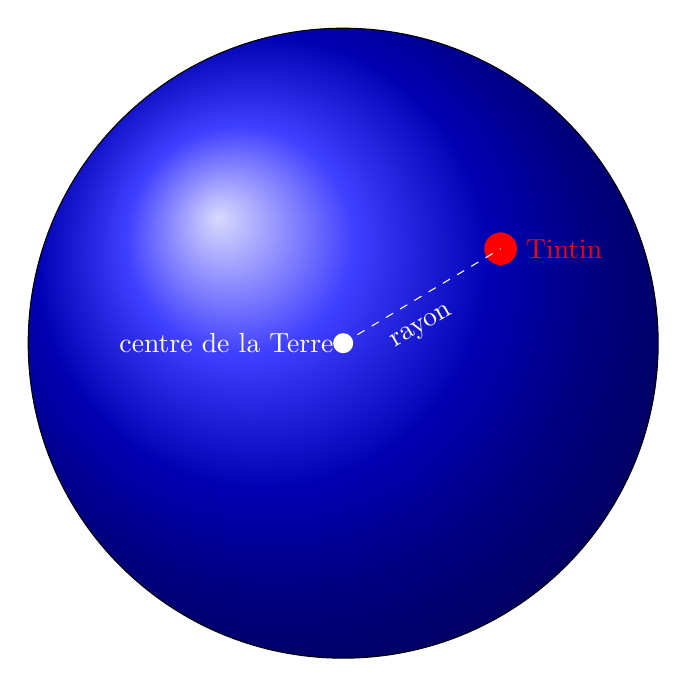
\begin{tikzpicture}[scale=4]
        \draw[fill=gray!50!white, shading=ball] (0,0) circle (1);
        \draw[red,fill=red] (0.5,0.3) circle (0.05);
        \draw[white,fill=white] (0,0) circle (0.03);
        \draw[white, dashed] (0,0) -- (0.5,0.3);
        \node[rotate=30, white] at (0.25,0.05) {rayon};
        \node[red,right,anchor=west] at (0.55,0.3) {Tintin};
        \node[white,left,anchor=east] at (0,0) {centre de la Terre};
    \end{tikzpicture}
\end{center}

On calcule : 
\begin{align*}
    F_{\mbox{Terre/Tintin}} &= G \times \dfrac{M_{\mbox{Terre}} \times M_{\mbox{Tintin}}}{{d_{\mbox{Terre/Tintin}}}^2} \\
    &= \num{6.67e-11} \times \dfrac{\num{6.0e24} \times \num{7.0e1}}{\left(\num{6.38e6}\right)^2} \\
    &= \left( \dfrac{\num{6.67} \times \num{6.0} \times \num{7.0}}{\num{6.38}^2} \right) \times \left( \dfrac{10^{-11} \times 10^{24} \times 10^1}{{10^6}^2} \right) \\
    &\approx \num{6.88} \times 10^{-11+24+1-2\times 6} \\
    &\approx \qty{6.88e2}{\newton}
\end{align*}

\clearpage
Quand on calcule $F_{\mbox{Terre/Tintin}}$, en fait on calcule le \emph{poids} de Tintin sur Terre. Pour cela, on peut utiliser une formule plus simple : 

\begin{align*}
    P_{\mbox{Tintin}} &= M_{\mbox{Tintin}} \times g \\
    &= \num{7.0e1} \times \num{9.8} \\ 
    &= \qty{686}{\newton} \\
    &= \qty{6.86e2}{\newton} ~~~~\mbox{(en écriture scientifique)}
\end{align*}

Qu'on utilise la première ou la deuxième formule, on obtiendra le même résultat.

Ensuite, il faut faire la même chose pour la Lune.


\end{document}